\documentclass[border=0mm]{standalone}

\usepackage{import}
\subimport{../../../}{preamble.tex}

\usepackage{tikz}
\usetikzlibrary{calc}
\usepackage{pgfplots}
\usepgfplotslibrary{fillbetween}

\renewcommand{\t}{-5}

\begin{document}

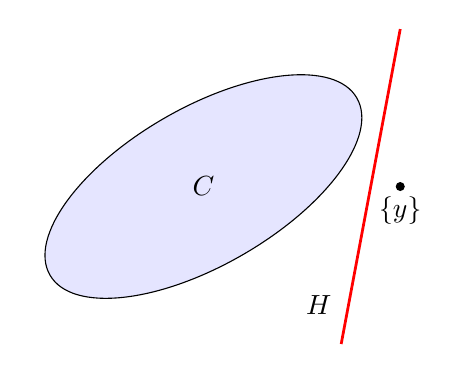
\begin{tikzpicture}[
  extended line/.style={shorten >=-#1},
  scale=0.5
  ]

  \begin{scope}[rotate=30]
    \coordinate (O) at (0,0);
    \coordinate (A) at (4.5,0);
    \coordinate (B) at (0,2);
    % draw ellipse
    \draw[black, fill=blue!10] (O) ellipse (4.5cm and 2.0cm);
    \node at (0,0) {$C$};
  \end{scope}

  \draw[line width=1pt, red] (3.5, -4) -- (5, 4);
  \node[left] at (3.5, -3) {$\red{H}$};

  \begin{scope}[xshift=5cm, yshift=1cm]
    \node[circle, fill=black, draw, inner sep=1] (D) at (0,-1) {};
    \node[below] at (D) {$\{y\}$};
  \end{scope}

\end{tikzpicture}

\end{document}

%%% Local Variables:
%%% mode: latex
%%% TeX-master: t
%%% End:
